
\documentclass[a4paper, 10pt]{article}  

\usepackage{geometry}
\geometry{a4paper, margin=1in}
    
\usepackage{verbatim}
\usepackage{graphicx}
\usepackage{pdfpages}
\usepackage{cite}
\usepackage{listings}
\usepackage{float}

\lstset{
	tabsize=2,
	breaklines=true
}

\setlength{\parskip}{1em}

\title{\LARGE \bf Project 1: Pneumatic Cylinder\\Mechatronics  282 778}
\author{Marc Alexander Sferrazza \\ 12164165
\thanks{This work was not supported by any organization}
\thanks{Faculty of Mechatronics Engineering, Massey University, Albany, Auckland, New Zealand
        {\tt\small Progress of project: https://github.com/alex1v1a/Mechatrnoics/} } }

\begin{document}

\maketitle

%\begin{figure}[H]
%  \includegraphics[width=\linewidth]{images/}
%  \label{fig:opencv}
%\end{figure}

\thispagestyle{empty}
\pagestyle{plain}


%%%%%%%%%%%%%%%%%%%%%%%%%%%%%%%%%%%%%%%%%%%%%%%%%%%%%%%%%%%%%%%%%%%%%%%%%%%%%%%%

\begin{abstract}

%A brief report on OpenCV to calculate spatial transformations. Each step was tested and an output image saved to the local folder. For a more detailed instruction on the stages not explained please review the source code in the appendix.

\end{abstract}


\clearpage
\tableofcontents
\listoffigures
%\listoftables
\thispagestyle{empty}
\clearpage

%%%%%%%%%%%%%%%%%%%%%%%%%%%%%%%%%%%%%%%%%%%%%%%%%%%%%%%%%%%%%%%%%%%%%%%%%%%%%%%%
%%%%%%%%%%%%%%%%%%%%%%%%%%%%%%%%%%%%%%%%%%%%%%%%%%%%%%%%%%%%%%%%%%%%%%%%%%%%%%%%

\setcounter{page}{1}

\section{INTRODUCTION}

%OpenCV (Open Source Computer Vision Library) is an open source machine learning library for visual components. It has been widely accepted as one of the worlds most used image processing tools, and has the capability of static and dynamic comprehension. Some of the basic features available in OpenCV are capable mapping environments to be used in demonstration such as self driving cars lane detection. 
%
%The process's aim in this project to achieve is to design a program in the Visual Studio environment, using the OpenCV library that will detect an characters location and find the work piece and its target location in a given workspace. The objective is to then calculate the distance and angle required to translate and rotate the work piece from its current location to it target location; and finally express the distance and angle as a homogeneous transform, and display the final results and image to the user, as described in the outline. 
%
%Unfortunately due to technical issues experienced, the final program has been compiled from source on a Mac with terminal. The shared and static lib's created in cmake then processed executables saved in the local library. Please note this when trying to re-compile as the some of the linkers may direct to other locations e.g. headers.
%
%OpenCV is a powerful tool for image processing with more then 2500 algorithms available in its library; by using several functions within the OpenCV library, a processed image will produce these values. 

%%%%%%%%%%%%%%%%%%%%%%%%%%%%%%%%%%%%%%%%%%%%%%%%%%%%%%%%%%%%%%%%%%%%%%%%%%%%%%%%
%%%%%%%%%%%%%%%%%%%%%%%%%%%%%%%%%%%%%%%%%%%%%%%%%%%%%%%%%%%%%%%%%%%%%%%%%%%%%%%%

\section{METHOD}

%A few images have been provided of different characters on a workspace and their corresponding transform locations. The process will involve filtering this image to a workable standard in which the contours can be used to formulate the translations and transformations from frames of workspaces. 
%
%As there are five images the option to run the process with all outputs was first made, but then the decision of what images to check was implemented using the case keys 1, 2, 3, 4, 5, esc - A prompt will be given to the user to select which image to process and find the balls with their colours; the user can cycle back to the main image selection and select another image to process. 
%
%The program can be closed by selecting the esc key from the prompt menu. This process helps break down the information for a simpler and more specific program allowing the user to choose their results accordingly.
%
%The image is then loaded to memory and with each step through the detection the image is saved for easy debugging, it also helps create a faster process and cleaner environment. 
%
%After the user has selected a desired image to process the transform function is called to preform the action. The sequence begins with the original image as shown below (set three from the five images are used for demo purposes in this report, as it was found one of the more complex)
%
%\begin{figure}[H]
%  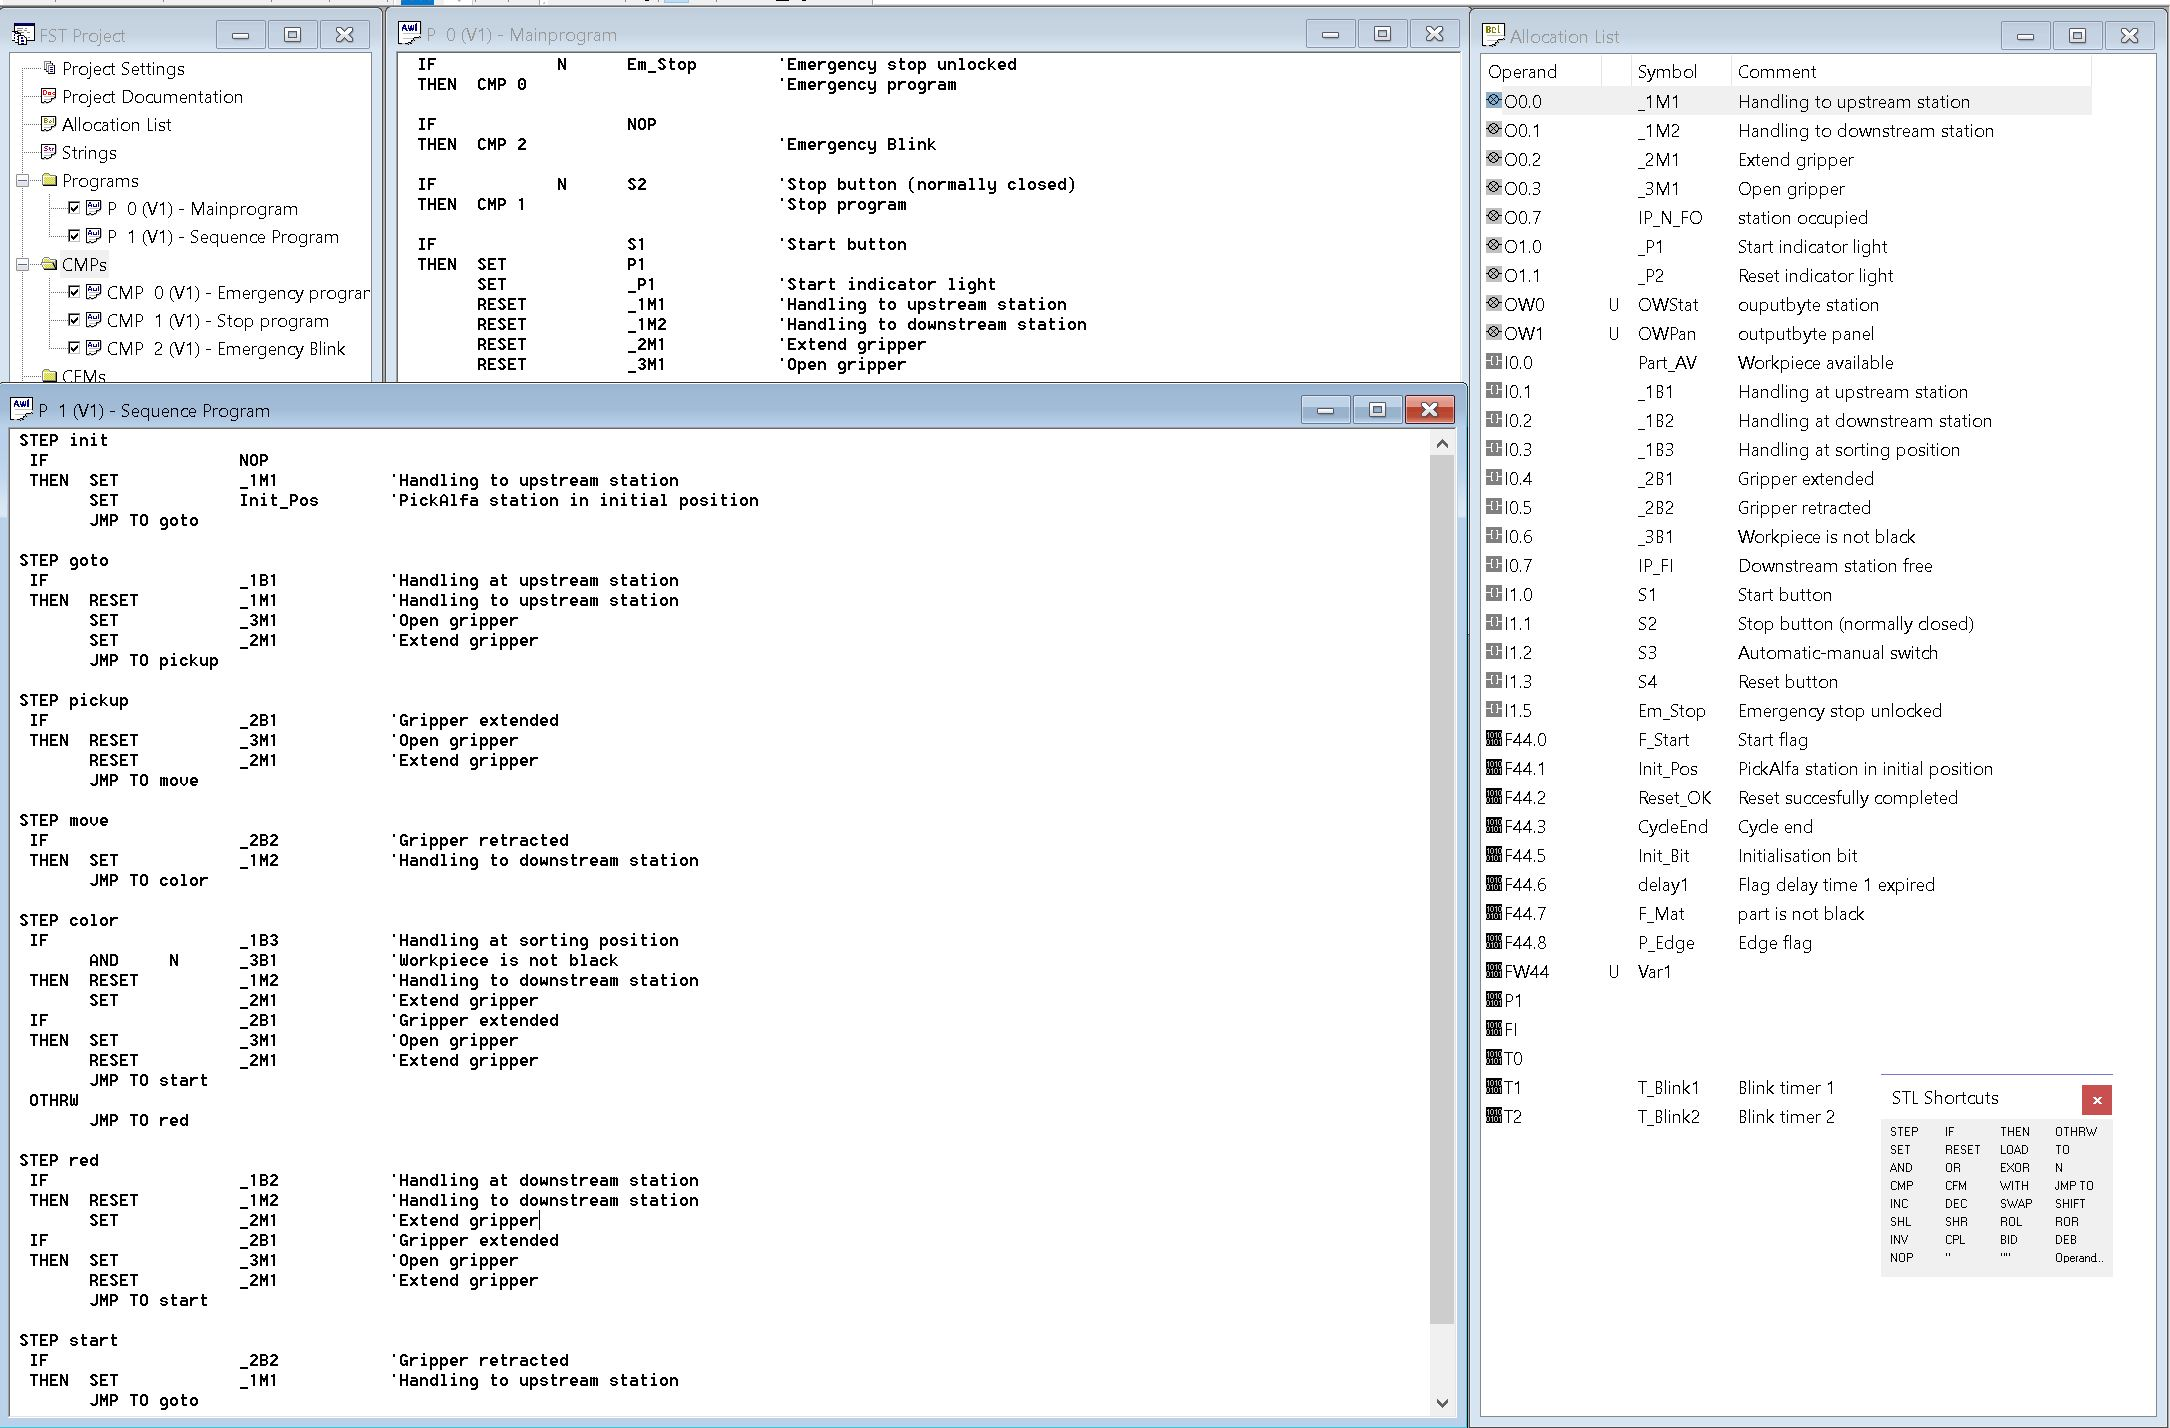
\includegraphics[width=\linewidth]{images/3}
%  \caption{Initial Image}
%  \label{fig:Initial Image}
%\end{figure}
%
%After the image has been processed and the workspace translated, and output is displayed of the resulting transformations; a homogenous matrix is also displayed.
%
%A full break down of the process has been attached and can be found in the code in the appendix. The following code is the process for user input and the function call for transform.

\begin{lstlisting}[language = C++]

\end{lstlisting}

%%%%%%%%%%%%%%%%%%%%%%%%%%%%%%%%%%%%%%%%%%%%%%%%%%%%%%%%%%%%%%%%%%%%%%%%%%%%%%%%

\subsection{BGR to HSV conversion}

%After the transform function has been called, the image is read into memory and resized for processing. In order to make the process more definite a conversion to greyscale is necessary, this will make the process more robust by converting a BGR. The greyscale conversion is ready to begin, using the cvtColor function to convert the image to greyscale (BGR2GRAY) will help in the detection processing.

\begin{lstlisting}[language = C++]

\end{lstlisting}

%%%%%%%%%%%%%%%%%%%%%%%%%%%%%%%%%%%%%%%%%%%%%%%%%%%%%%%%%%%%%%%%%%%%%%%%%%%%%%%%

\subsection{Gaussian Blur}

%The Gaussian blur is used to reduce the noise of the image and smoothing the edges to help eliminate any external influences when finding the shape and give a more accurate average of the pixels. The function will transform the image using convolution matrix Gaussian kernel, and will give a result based on each pixel and it's surrounding pixels to contour and blur while maintaining the edges integrity.
%
%After the Gaussian process, the image is passed to the canny operator for edge detection. The best values for Gaussian used are a 3x3 kernel matrix with a standard deviation of 1.

\begin{lstlisting}[language = C++]

\end{lstlisting}

%%%%%%%%%%%%%%%%%%%%%%%%%%%%%%%%%%%%%%%%%%%%%%%%%%%%%%%%%%%%%%%%%%%%%%%%%%%%%%%%

\subsection{Canny edge detection}

%The Gaussian blur Canny edge detection function is then called to preform detection for the workspace. The frames are assessed from the greyscale smooth edged original image, and the output is assigned to out threshold image space.
% 
%After the canny edge detection the image is then passed though a dilation and erosion functions to reduce noise.

\begin{lstlisting}[language = C++]

\end{lstlisting}

%%%%%%%%%%%%%%%%%%%%%%%%%%%%%%%%%%%%%%%%%%%%%%%%%%%%%%%%%%%%%%%%%%%%%%%%%%%%%%%%

\subsection{Dilation \& Erosion}

%Using the dilation function the image begins to form more solid shapes and removes discrepancies to better form solid filled in shapes, by adding pixels to the boundaries found of objects and shapes in a greyscale image. The erosion function then emphasises those shapes making it easier for the shape identifier later on by removing pixels from the boundaries of objects. The best values found for the size of the morphological operations are as shown below.

\begin{lstlisting}[language = C++]

\end{lstlisting}

%%%%%%%%%%%%%%%%%%%%%%%%%%%%%%%%%%%%%%%%%%%%%%%%%%%%%%%%%%%%%%%%%%%%%%%%%%%%%%%%

\subsection{Contours}

%This algorithm finalises the edge detection and creates fine line edges for rotating the rectangles. After all the vectors containing contours are stored, and the hierarchy datatype is linked, when the function is called the parent and child contours are stored respectivly.
%
%The algorithm finds the rectangles of each outline (character) which subsequently is used to establish the orientation by using the vertices of the contour, and in turn find the difference in angle for each object. The output of this process gives two vectors that contains instances as elements the same size of the vectors of that from contour. The significant points are then recorded to the vector matrices to find the spacial transformations. 

\begin{lstlisting}[language = C++]

\end{lstlisting}

%%%%%%%%%%%%%%%%%%%%%%%%%%%%%%%%%%%%%%%%%%%%%%%%%%%%%%%%%%%%%%%%%%%%%%%%%%%%%%%%

\subsection{Bounding Rectangles \& Approximate Contours to Polygons}

%Bounding for a particular object rectangle converts the contour to a polygon shape. The vector is that of the same size of the contour vector, but is declared to address the points of each rectangle. The algorithm used converts the bounding rectangles to a polygon shape.

\begin{lstlisting}[language = C++]

\end{lstlisting}

%%%%%%%%%%%%%%%%%%%%%%%%%%%%%%%%%%%%%%%%%%%%%%%%%%%%%%%%%%%%%%%%%%%%%%%%%%%%%%%%

\subsection{Drawing Contours, Rotated Rectangles \& Center circles with Axis}

%In this process an image is then created to find the spacial transforms. The first step is to save all the points required to the image, then draw them on the final image. The process involves using contrasts to find contour lines, then looping to draw the contour lines and rectangles accordingly. The center and translation lines are then drawn to establish the difference between the two rectangles and find the coordinates for each contour.

\begin{lstlisting}[language = C++]

\end{lstlisting}

%%%%%%%%%%%%%%%%%%%%%%%%%%%%%%%%%%%%%%%%%%%%%%%%%%%%%%%%%%%%%%%%%%%%%%%%%%%%%%%%

\subsection{Translation}

%As the z axis is ignored in this instance the x and y axis are observed to find the translation difference of the two center points of the rectangles. Using Pythagoras's trigonometry equations with the established center points a subsidy can be made to suit the algorithm and simply find the difference of the characters. Then to rotate the character it is first found between a positive or negative 180 degree value, and in the clockwise or anticlockwise direction. The angles are found for each set of 90 degrees passed, then adjusted accordingly.

\begin{lstlisting}[language = C++]

\end{lstlisting}

%%%%%%%%%%%%%%%%%%%%%%%%%%%%%%%%%%%%%%%%%%%%%%%%%%%%%%%%%%%%%%%%%%%%%%%%%%%%%%%%
%%%%%%%%%%%%%%%%%%%%%%%%%%%%%%%%%%%%%%%%%%%%%%%%%%%%%%%%%%%%%%%%%%%%%%%%%%%%%%%%

\section{RESULTS}

%After the processing is complete the original image is displayed, and terminal output response given; The final result is shown below. The process is successful and the workspace transformation is complete. The user can now press any key to go back and select another image, or after closing the image hit the "esc" key to exit the program.

\begin{lstlisting}[language = C++]

\end{lstlisting}

%\begin{figure}[H]
%  \includegraphics[width=\linewidth]{images/F3}
%  \caption{The final image is given with workspace results}
%  \label{fig:The final image is given with workspace results}
%\end{figure}
%
%After the transformation and translation of the frames the final image is saved to the local output folder, per process, the center coordinates, homogeneous transformation matrix, rotation and translation between characters are all displayed to the user as output in terminal. A sample of the results can be seen below.
%
%\begin{figure}[H]
%  \includegraphics[width=\linewidth]{images/shell}
%  \caption{The final results shown of the output: center coordinates, homogeneous transformation matrix, rotation and translation between characters}
%  \label{fig:Final Results Shell}
%\end{figure}

%%%%%%%%%%%%%%%%%%%%%%%%%%%%%%%%%%%%%%%%%%%%%%%%%%%%%%%%%%%%%%%%%%%%%%%%%%%%%%%%
%%%%%%%%%%%%%%%%%%%%%%%%%%%%%%%%%%%%%%%%%%%%%%%%%%%%%%%%%%%%%%%%%%%%%%%%%%%%%%%%

\section{OUTCOMES}

%%%%%%%%%%%%%%%%%%%%%%%%%%%%%%%%%%%%%%%%%%%%%%%%%%%%%%%%%%%%%%%%%%%%%%%%%%%%%%%%

\subsection{Fine Tuning} 

%While the process is consistent it is a clear underling of step by step operations, the procedure in which was either suitable or inadequate. This involves checking the matrix at different points like the threshold values, dilation and erosion, the Gaussian blur, and in particular the vectors and contours for find bounding rects, circles, and approximate contours to polygons, translation and transforms of each frame and combine workspace.

%%%%%%%%%%%%%%%%%%%%%%%%%%%%%%%%%%%%%%%%%%%%%%%%%%%%%%%%%%%%%%%%%%%%%%%%%%%%%%%%

\subsection{Testing}

%Ensure the target of finding translation from frames are complete and accurate, checking each function independently for a robust break down and good debugging.
%
%Each step had an output image saved to check the processes respectively. The images are checked to make sure each stage is completing the task correctly, if not the code is then referred to and further revisions are made.
%
%Every image was tested with the values for recognition and tweaked in the fine tuning process to get the best possible results.

%%%%%%%%%%%%%%%%%%%%%%%%%%%%%%%%%%%%%%%%%%%%%%%%%%%%%%%%%%%%%%%%%%%%%%%%%%%%%%%%

\subsection{Finalising}

%After all the results were finalised and correct the outputs and results confirmed the code was then stripped and simplified for clarity and ease of use for future development and reference.
%
%Making the program stable and concise, and as robust as possible builds for a good design. Checking over the functions and any redundant code, ensure a good user interface is easily workable and the outputs are all correct and comprehensive.

%%%%%%%%%%%%%%%%%%%%%%%%%%%%%%%%%%%%%%%%%%%%%%%%%%%%%%%%%%%%%%%%%%%%%%%%%%%%%%%%
%%%%%%%%%%%%%%%%%%%%%%%%%%%%%%%%%%%%%%%%%%%%%%%%%%%%%%%%%%%%%%%%%%%%%%%%%%%%%%%%
\clearpage
\section{CONCLUSIONS}

\subsection{Critical Evaluation and Methodology}

%The final transformation of workspaces have been produced from several steps. This demonstration gives the user a guided input and accurate clear output for, easy to use, and self guided results.
%
%As the output for all processed images was found accurate and complete the method has been found effective. The results are clearly given show the center coordinates of both contours, a homogeneous transformation matrix, rotation and translation between characters all displayed to the user as output in terminal, and the final image saved to the output source folder. 

\subsection{Discussion}

%This process preforms and meets all aims and objects set out to achieve and can be considered a success. All required information displayed to the user in an orderly fashion and input methods are acceptable. In achieving this task the demonstration presents a practical form in which by using bounding rectangles, contours and points vectors, a total accurate reformation can be drawn accross a translational span.
%
%The process's used were successfully able to detect and identify all characters, and have been able to take the product of matrices and find significant angles. The transformations have completed all images with speed and accuracy, and is a viable method of detection and transformation.

%%%%%%%%%%%%%%%%%%%%%%%%%%%%%%%%%%%%%%%%%%%%%%%%%%%%%%%%%%%%%%%%%%%%%%%%%%%%%%%%
%%%%%%%%%%%%%%%%%%%%%%%%%%%%%%%%%%%%%%%%%%%%%%%%%%%%%%%%%%%%%%%%%%%%%%%%%%%%%%%%

\nocite{*}
\bibliographystyle{ieeetr}
\bibliography{references}

%%%%%%%%%%%%%%%%%%%%%%%%%%%%%%%%%%%%%%%%%%%%%%%%%%%%%%%%%%%%%%%%%%%%%%%%%%%%%%%%
%%%%%%%%%%%%%%%%%%%%%%%%%%%%%%%%%%%%%%%%%%%%%%%%%%%%%%%%%%%%%%%%%%%%%%%%%%%%%%%%

\clearpage
\section*{APPENDIX}

\begin{lstlisting}[language = C++]

\end{lstlisting}

\end{document}
